\documentclass{article}
\usepackage{amsmath}
\usepackage{tikz}
\tikzstyle{every picture}+=[remember picture]
\usetikzlibrary{matrix}

\usepackage{gauss2}
% patch gauss macros for doing their work in `align'
% and other amsmath environments; see
% http://tex.stackexchange.com/questions/146532/
\usepackage{etoolbox}
\makeatletter
\patchcmd\g@matrix
 {\vbox\bgroup}
 {\vbox\bgroup\normalbaselines}% restore the standard baselineskip
 {}{}

\newdimen\colwidth
\def\arrowheight{\g@dim{cx1}{\colwidth}}
\newdimen\rowheight
\def\arrowwidth{\g@dim{cy1}{\rowheight}}
\def\gvline{\g@vline}
\newdimen\sumen
\let\gsetdim=\g@defdim
\let\gmaxcol=\g@maxcol
\let\gmaxrow=\g@maxrow
\let\gdouble=\g@double
\let\gdefdouble=\g@defdouble
\let\gadvance=\g@advance
\let\gdim=\g@dim
\let\gdist=\g@dist
\let\gdistD=\g@distD
\let\gtmpb=\g@d@tmpb

\newbox\g@centerbox

\def\g@center{%
  \g@endregion% wenn das erste Mal g@endregion in matrixdivs, colops oder rowops aufgerufen wird, ist es gleich g@endmatrix. Dort wird die g@matrixbox gebaut
  \gdef\matrixdivs{\PackageError{gauss}{Two sets of matrix dividers are spedified in just one matrix. This is not allowed.}}%
  \gdef\g@endregion{%
    \end{picture}\egroup
    \g@measureArea{cy}{0}{\the\g@maxcol}{sum}%
    \g@dim{sum}{\ht\g@centerbox}%
    \global\setbox\g@centerbox=\hbox{%
      \box\g@centerbox%
    }%
  }
  \g@defdim{sum}{\z@}
  \global\setbox\g@centerbox=\hbox\bgroup
    \begin{picture}(\g@double{w},0)(0,0)
      \linethickness{\g@linethickness}
}

% new matrix environment
\newenvironment{gmatrixex}[1][]
{\unitlength=1pt\def\g@environment{#1matrix}%
 \begin{g@matrixex}%
}{%
 \end{g@matrixex}%
 \let\matrix\@empty
 \let\endmatrix\@empty
 \g@d@tmpa\ht\g@matrixbox \advance\g@d@tmpa\p@% change \p@ to <x>pt when another spacing to the top and bottom is wanted
 \g@d@tmpb\dp\g@matrixbox \advance\g@d@tmpb\p@% change \p@ to <x>pt when another spacing to the top and bottom is wanted
 \g@d@tmp\ht\g@northbox \ht\g@northbox\z@
 \dp\g@northbox\z@
 \ifdim \g@d@tmp>\z@
  \advance\g@d@tmp-\opskip
 \fi
 \advance\g@d@tmp.5\ht\g@matrixbox
 \advance\g@d@tmp.5\dp\g@matrixbox
 \begin{\g@environment}%
  %\rule{5pt}{\z@}% CHANGE: So kann Abstand zu den Klammern eingeführt werden
  \vcenter{\hbox{% vcenter, da sonst alles in relation zu baseline positioniert wird
   %CHANGE \rlap{\raise\ht\g@matrixbox\box\g@northbox}% north
   \rlap{%
    \g@dim{d}{\g@d@tmpa}% to keep the chance to tmpa local
    \lower\g@d@tmpa\box\g@centerbox% lowering is needed for the right alignment => WHY NEEDED? How does the depth play into alignment with \vcenter?
    }%
    \rlap{%
      \raise\ht\g@matrixbox\box\g@northbox% lowering is needed for the right alignment
    }%
   % 1 additional pt above and below the matrix
   % \z@ is just a dimension of 0.0pt
   % \g@d@tmpa is the height of the width-zero rule
   % it is set ot the height of the matrixbox
   \rule\z@\g@d@tmpa%
   % lower an empty box by the depth of the matrixbox
   \lower\g@d@tmpb\null%
   \box\g@matrixbox% the matrix itself
  }}%
  %\rule{5pt}{\z@}% CHANGE: So kann Abstand zu den Klammern eingeführt werden
  \end{\g@environment}%
  \rule{\rowarrowsep}{\z@}% adds space to the right of the right paranthese 
  % \g@d@tmp has the length of height of the northbox + half the height of the matrix (as it is aligned centered wrt the baseline) + half the depth of the matrix
  \rule{\z@}{\g@d@tmp}% this rule is placed at the baseline of the equation
  \g@dim{d}{\g@d@tmpa}%
  \vcenter{\hbox{\lower\g@d@tmpa\box\g@eastbox}}%
}

\edef\g@prae{\hfil\noexpand\mathstrut$\relax}
\edef\g@post{\relax$\hfil} 
\newenvironment{g@matrixex}
{\setbox\g@trash=\hbox\bgroup
  \global\g@maxrow@old\g@maxrow
  \global\g@maxcol@old\g@maxcol
  \global\g@maxrow0%
  \global\g@maxcol0%
  \let\rowops\g@east
  \let\colops\g@north
  \let\matrixdivs\g@center
  \vbox\bgroup%
    \normalbaselines% fix spacing for align environments
    % count rows while typesetting
    \def\\{% needed to get redefined: \cr needs to come last so vertical spacing can be inserted with \noalign{\vskip <x>pt}
      \mathstrut%
      \global\advance\g@maxrow1\relax%
      \cr%
    }%
    \global\let\g@endregion\g@endmatrix
    \global\g@tab=2\arraycolsep
    \ialign\bgroup\g@prae##\g@post&&\kern\g@tab\g@prae##\g@post\cr
}{%
  \g@endregion
  \egroup % end of \hbox which is put into g@trash in g@endmatrix or the north-, east- or centerbox from g@north, g@east or g@center
  % enable nested gmatrixes (for DniQ :-)
  \global\g@maxrow\g@maxrow@old
  \global\g@maxcol\g@maxcol@old
  \global\let\g@endregion\g@endmatrix
  \global\let\rowops\g@east
  \global\let\colops\g@north
}

%\edef\g@post{\relax$} % $ 

\makeatother
 
\newcommand{\BAR}{%
  \hspace{-\arraycolsep}%
  \strut\vrule % the `\vrule` is as high and deep as a strut
  \hspace{-\arraycolsep}%                 
}
\def\rowaddtolabel#1{\scriptscriptstyle #1}
\def\coladdtolabel#1{\scriptscriptstyle #1}

\begin{document}
Hello Gordon, how are you? 
\begin{align*}
  A = \begin{gmatrixex}[p]
    4&3&5 & 1&0\\ 
    5&333333&5  &0&-1 \\
    \noalign{\vskip0.5\baselineskip}
    -1&0&0&\\
    0&1&0&\\
    0&\displaystyle\sum_{i=1}^n i^2&1b& & 
    \matrixdivs 
    %\add[-1]{0}{4}
    \arrowheight
    %\divide\colwidth by 2
    %\tikz[overlay]{\draw (a)+(-\the\colwidth,0) -- (b);}
    \arrowwidth
    \divide\rowheight by 2
    %\tikz[overlay]{\draw (ad)+(0,\the\rowheight)--(bd)}
    \newdimen\zz
    \setlength{\zz}{0cm}
    \gsetdim{zz}{\zz}
    \setlength{\sumen}{-2cm}
    \gsetdim{sumen}{\sumen}
    %\gvline{cx3}{ry\the\gmaxrow}{sumen}%{ry\the\gmaxrow}
    %\put(\gdouble{cx3},-\gdouble{ry\the\gmaxrow}){\line(0,-1){\gdouble{ry0}}}
    %\put(0,-\gdouble{diff}){\line(1,0){\gdouble{cx\the\gmaxcol}}}
    \newdimen\matrixwidth
    \gdim{w}{\matrixwidth}
    \gdefdouble{innermatrixwidth}{\matrixwidth}
    %\put(0,-\gdouble{diff}){\line(1,0){\gdouble{innermatrixwidth}}}
    \newdimen\matrixheight
    \gdim{h}{\matrixheight}
    \gdefdouble{innermatrixheight}{\matrixheight}
    %\put(\gdouble{cx3},-\gdouble{ry\the\gmaxrow}){\line(0,-1){\gdouble{innermatrixheight}}}
    \newdimen\diff
    \newdimen\temp
    \gdim{rb\the\gmaxrow}{\diff}
    \gdim{d}{\temp}
    \advance\diff -0.5\temp
    \gdefdouble{vdivbaseline}{\diff}
    \put(\gdouble{cm3},\gdouble{vdivbaseline}){\line(0,1){\gdouble{innermatrixheight}}} % vertical divider
    %\put(\gdouble{cx3},\gdouble{rb\the\gmaxrow}){\line(0,1){\gdouble{innermatrixheight}}}
    %\put(\gdouble{cx2},\gdouble{rb\the\gmaxrow}){\line(0,1){\gdouble{innermatrixheight}}}
    %
    \gdim{rb1}{\diff}
    \gdim{rt2}{\temp}
    \advance\diff -\temp
    \advance\diff -0.5\diff
    \advance\diff\temp
    \gdefdouble{midliney}{\diff}
    \put(0,\gdouble{midliney}){\line(1,0){\gdouble{innermatrixwidth}}} % horiziontal divider
    %\put(0,\gdouble{rb1}){\line(1,0){\gdouble{innermatrixwidth}}}
    %\put(0,\gdouble{rt2}){\line(1,0){\gdouble{innermatrixwidth}}}
    \put(0,\gdouble{rb\the\gmaxrow}){\color[rgb]{1,0,0}\line(1,0){\gdouble{innermatrixwidth}}}
    \put(0,0){\color[rgb]{0,1,0}\line(1,0){\gdouble{innermatrixwidth}}}
    %\put(\gdouble{cx2},\gdouble{rt0}){\line(0,1){\gdouble{d}}}
    \put(0,\gdouble{rt0}){\color[rgb]{1,0,0}\line(1,0){\gdouble{innermatrixwidth}}}
    %
    \rowops 
    \add[-1]{0}{4}
    \put(0,0){\color[rgb]{1,0,0}\line(1,0){80}}
    \colops
    \add[2]{1}{3}
    \add[-3]{0}{2}
  \end{gmatrixex} 
\end{align*}
I am just very fine, thank you for asking. 
\ialign{
    # & \hfil # \hfil \cr
    Erste Zeile\cr% Fügt eine horizontale Linie ein
    Zweite Zeile \cr
}

\begin{align}
  \begin{gmatrix}[p]
    4&3&5 & 1&0\\ 
    5&333333&5  &0&-1 \\
    -1&0&0&\\
    0&1&0&\\
    0&\sum_{i=1}^n i^2&1b& & 
    \colops 
    %\add[-1]{0}{4}
    \arrowheight
    %\divide\colwidth by 2
    %\tikz[overlay]{\draw (a)+(-\the\colwidth,0) -- (b);}
    \arrowwidth
    \divide\rowheight by 2
    %\tikz[overlay]{\draw (ad)+(0,\the\rowheight)--(bd)}
    \newdimen\zz
    \setlength{\zz}{0cm}
    \gsetdim{zz}{\zz}
    \setlength{\sumen}{-2cm}
    \gsetdim{sumen}{\sumen}
    %\gvline{cx3}{ry\the\gmaxrow}{sumen}%{ry\the\gmaxrow}
    %\put(\gdouble{cx3},-\gdouble{ry\the\gmaxrow}){\line(0,-1){\gdouble{ry0}}}
    %\put(0,-\gdouble{diff}){\line(1,0){\gdouble{cx\the\gmaxcol}}}
    \newdimen\matrixwidth
    \gdim{w}{\matrixwidth}
    \gdefdouble{innermatrixwidth}{\matrixwidth}
    %\put(0,-\gdouble{diff}){\line(1,0){\gdouble{innermatrixwidth}}}
    \newdimen\matrixheight
    \gdim{h}{\matrixheight}
    \gdefdouble{innermatrixheight}{\matrixheight}
    %\put(\gdouble{cx3},-\gdouble{ry\the\gmaxrow}){\line(0,-1){\gdouble{innermatrixheight}}}
    \put(\gdouble{cm3},0){\line(0,1){\gdouble{innermatrixheight}}}
    %
    \newdimen\diff
    \gdim{rb1}{\diff}
    \newdimen\temp
    \gdim{rt2}{\temp}
    \advance\diff -\temp
    \advance\diff -0.5\diff
    \advance\diff\temp
    \gdefdouble{midliney}{\diff}
    \put(0,\gdouble{midliney}){\line(1,0){\gdouble{innermatrixwidth}}}
    %\put(0,\gdouble{rb1}){\line(1,0){\gdouble{innermatrixwidth}}}
    %\put(0,\gdouble{rt2}){\line(1,0){\gdouble{innermatrixwidth}}}
    %
    \rowops 
    \add[-1]{0}{4}
  \end{gmatrix} 
\end{align}

\begin{align}
  \begin{gmatrix}[p]
    4&3&5 & &1 \\ 
    5&3&5 & &0
    \colops 
    %\add[-1]{0}{4}
    \arrowheight
    %\divide\colwidth by 2
    %\tikz[overlay]{\draw (a)+(-\the\colwidth,0) -- (b);}
    \arrowwidth
    \divide\rowheight by 2
    %\tikz[overlay]{\draw (ad)+(0,\the\rowheight)--(bd)}
    \newdimen\zz
    \setlength{\zz}{0cm}
    \gsetdim{zz}{\zz}
    \setlength{\sumen}{-2cm}
    \gsetdim{sumen}{\sumen}
    %\gvline{cx3}{ry\the\gmaxrow}{sumen}%{ry\the\gmaxrow}
    %\put(\gdouble{cx3},-\gdouble{ry\the\gmaxrow}){\line(0,-1){\gdouble{ry0}}}
    %\put(0,-\gdouble{diff}){\line(1,0){\gdouble{cx\the\gmaxcol}}}
    \newdimen\matrixwidth
    \gdim{w}{\matrixwidth}
    \gdefdouble{innermatrixwidth}{\matrixwidth}
    %\put(0,-\gdouble{diff}){\line(1,0){\gdouble{innermatrixwidth}}}
    \newdimen\matrixheight
    \gdim{h}{\matrixheight}
    \gdefdouble{innermatrixheight}{\matrixheight}
    \newdimen\temp
    \gdim{ry2}{\temp}
    \newdimen\diff
    \setlength\diff\matrixheight
    \advance\diff -\temp
    \gdefdouble{diffe}{\diff}
    %\put(\gdouble{cx3},-\gdouble{ry\the\gmaxrow}){\line(0,-1){\gdouble{innermatrixheight}}}
    \put(\gdouble{cx3},0){\line(0,1){\gdouble{innermatrixheight}}}
    %\put(0,\gdouble{ry2}){\line(1,0){\gdouble{innermatrixwidth}}}
    \rowops 
    \add[-1]{0}{1}
  \end{gmatrix} 
\end{align}

\begin{align*}
  \left(\begin{array}{ccc|cc}
    4&3&5 & 1&0\\ 
    5&3&5 & 0&-1\\ 
    \hline
    -1&0&0&\\
    0&1&0&\\
    0&0&1b 
  \end{array}\right)
\end{align*}

Hello Gordon, how are you?
\begin{align*}
&\begin{gmatrix}[p]4&3&4&\BAR& 1&0\\ 5&3&5 &\BAR &0&1\vspace{-2mm}\\ \tikz{\coordinate (a) at (0,0)} & & & & & \tikz{\coordinate (b) at (0,0)}\tikz[overlay]{\draw (a) -- (b);} \\ 1&0&0&\BAR\\0&1&0&\BAR\\0&0&1&\BAR \colops \add[-1]{0}{2}\end{gmatrix} 
\longrightarrow \begin{gmatrix}[p]4&3&0&\BAR& 1&0\\5&3&0 &\BAR &0&1 \vspace{-2mm}\\ \rule{28mm}{0.5pt} \hspace{-25mm} \\  1&0&-1&\BAR\\0&1&0&\BAR\\0&0&1&\BAR \colops \add[-1]{1}{0} \end{gmatrix} 
\longrightarrow \begin{gmatrix}[p]1&3&0&\BAR& 1&0\\2&3&0 &\BAR &0&1\vspace{-2mm}\\ \rule{32mm}{0.5pt} \hspace{-26mm} \\  1&0&-1&\BAR\\-1&1&0&\BAR\\0&0&1&\BAR \rowops \add[-2]{0}{1} \end{gmatrix} \\[2mm]
&\longrightarrow \begin{gmatrix}[p]1&3&0&\BAR& 1&0\\0&-3&0 &\BAR &-2&1\vspace{-2mm}\\ \rule{35mm}{0.5pt} \hspace{-32mm} \\  1&0&-1&\BAR\\-1&1&0&\BAR\\0&0&1&\BAR \rowops \add[+1]{1}{0} \mult{1}{\cdot (-1)} \end{gmatrix} 
\longrightarrow \begin{gmatrix}[p]1&0&0&\BAR& -1&1\\0&3&0 &\BAR &2&-1\vspace{-2mm}\\ \rule{35mm}{0.5pt} \hspace{-32mm} \\  1&0&-1&\BAR\\-1&1&0&\BAR\\0&0&1&\BAR \end{gmatrix} \vspace{5mm}
\end{align*}
I am very fine, thank you for asking. 

Hallo \tikz[baseline]{\coordinate (ca) at (0,0);} wie geht es dir heute \tikz[baseline]{\coordinate (cb) at (0,0);}. 
\tikz[overlay]{\draw (ca) -- (cb);}

\begin{equation*}
    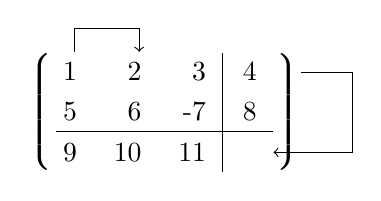
\begin{tikzpicture}[baseline]
        \matrix [
          matrix of math nodes,
          left delimiter={\lgroup},right delimiter={\rgroup},
          nodes in empty cells,
          nodes={inner xsep=0.25em,inner ysep = 0.4em, align=right, anchor=east},
          inner sep=0pt, column sep=.5em,
          %nodes={inner xsep = .2cm, inner ysep = .3cm}
        ] (m) {
         1 & 2 & 3 & 4 \\
         5 & 6 & -7 & 8 \\
         \hline
         9 & 10 & 11 &  \\
        } ;

        \draw (m-1-3.east)+(0,.25) -- (m-3-3.east) -- +(0,-0.25);
      
        \draw[->] (m-1-1.north) -- +(0,.3) -| (m-1-2.north);
        \draw[->] (m-1-4.east)+(1em,0) -- +(1,0) |- (m-3-4.east);
    \end{tikzpicture}
\end{equation*}

\end{document}
